% The Somnial Study - CSU Chico Capstone Poster
% Fall 2025

\documentclass[final]{beamer}

% ====================
% Poster Setup - 48x36 inches (standard)
% ====================
\usepackage[size=custom,width=121.92,height=91.44,scale=1.0]{beamerposter}

\usetheme{default}
\usecolortheme{default}

% ====================
% Packages
% ====================
\usepackage[T1]{fontenc}
\usepackage[utf8]{inputenc}
\usepackage{helvet}
\renewcommand{\familydefault}{\sfdefault}
\usepackage{graphicx}
\usepackage{booktabs}
\usepackage{tikz}
\usepackage{tcolorbox}
\usepackage{fontawesome5}
\usepackage{hyperref}
\usepackage{ragged2e}
\usepackage{enumitem}

\tcbuselibrary{skins,breakable}
\usetikzlibrary{positioning,shapes,arrows}

% ====================
% CSU Chico Colors
% ====================
\definecolor{chicomaroon}{RGB}{153,0,51}
\definecolor{chicogray}{RGB}{89,89,89}
\definecolor{chicolightgray}{RGB}{230,230,230}
\definecolor{chicowhite}{RGB}{255,255,255}
\definecolor{textdark}{RGB}{40,40,40}
\definecolor{dreampurple}{RGB}{75,50,110}
\definecolor{dreamcyan}{RGB}{70,160,190}

\setbeamercolor{background canvas}{bg=chicolightgray}

% ====================
% Custom Block Style - Matching CSU Chico format
% ====================
\newtcolorbox{posterblock}[1][]{
  enhanced,
  colback=chicowhite,
  colframe=chicomaroon,
  colbacktitle=chicomaroon,
  coltitle=white,
  fonttitle=\bfseries\LARGE,
  boxrule=0pt,
  arc=0pt,
  left=12pt,
  right=12pt,
  top=10pt,
  bottom=10pt,
  toptitle=8pt,
  bottomtitle=8pt,
  titlerule=0pt,
  title=#1,
  drop shadow={opacity=0.15}
}

\newtcolorbox{featurebox}{
  enhanced,
  colback=chicowhite,
  colframe=chicolightgray,
  boxrule=1pt,
  arc=0pt,
  left=8pt,
  right=8pt,
  top=6pt,
  bottom=6pt
}

% ====================
% Remove navigation
% ====================
\setbeamertemplate{navigation symbols}{}

% ====================
% Column dimensions
% ====================
\newlength{\sepwidth}
\newlength{\colwidth}
\setlength{\sepwidth}{0.015\paperwidth}
\setlength{\colwidth}{0.30\paperwidth}

\newcommand{\separatorcolumn}{\begin{column}{\sepwidth}\end{column}}

% ====================
% Graphics path
% ====================
\graphicspath{{./}}

% ====================
% Document
% ====================
\begin{document}

\begin{frame}[t]

% ====================
% HEADER with CSU Chico Logo and Title Banner
% ====================
\begin{tikzpicture}[remember picture,overlay]
  % Light gray header background
  \fill[chicolightgray] (current page.north west) rectangle ([yshift=-16cm]current page.north east);

  % CSU Chico Logo (top left)
  \node[anchor=north west] at ([xshift=2cm,yshift=-1cm]current page.north west) {
    
\includegraphics[height=8cm]{CSU Chico Logo.png}
  };

  % Title Banner (ribbon style)
  \fill[chicogray] ([xshift=25cm,yshift=-2cm]current page.north west) --
                   ([xshift=95cm,yshift=-2cm]current page.north west) --
                   ([xshift=97cm,yshift=-5cm]current page.north west) --
                   ([xshift=95cm,yshift=-8cm]current page.north west) --
                   ([xshift=25cm,yshift=-8cm]current page.north west) --
                   ([xshift=23cm,yshift=-5cm]current page.north west) -- cycle;

  % Project Title
  \node[white,font=\fontsize{64}{72}\selectfont\bfseries]
    at ([xshift=60cm,yshift=-5cm]current page.north west)
    {THE SOMNIAL STUDY};

  % Subtitle
  \node[chicogray,font=\fontsize{28}{32}\selectfont\itshape]
    at ([xshift=60cm,yshift=-9.5cm]current page.north west)
    {A First-Person Narrative Horror Experience};

  % Author Name
  \node[chicogray,font=\fontsize{36}{42}\selectfont\bfseries]
    at ([xshift=60cm,yshift=-12cm]current page.north west)
    {MUSTAFA ALI};

  % Semester (top right)
  \node[anchor=north east,chicomaroon,font=\fontsize{42}{48}\selectfont\bfseries]
    at ([xshift=-3cm,yshift=-3cm]current page.north east)
    {FALL 2025};

\end{tikzpicture}

\vspace{14cm}

% ====================
% CONTENT COLUMNS
% ====================
\begin{columns}[t]
\separatorcolumn

% =========================================
% COLUMN 1 - Overview & Languages/Tools
% =========================================
\begin{column}{\colwidth}

\begin{posterblock}[Overview]
\large
\justifying
\textbf{The Somnial Study} is a first-person narrative horror game I'm building in Unity, set in a distant future where humanity has developed interstellar travel.

\vspace{0.8cm}
A catastrophic meteor threatens Earth, forcing humanity to flee the solar system. The player attempts to escape but gets \textbf{abducted by aliens} who possess technology that can \textit{simulate and observe human dreams}---though they cannot control them.

\vspace{0.8cm}
Players experience multiple dream sequences that shift in tone---from euphoric to anxious to complete breakdown---as the aliens study the human mind and reality becomes increasingly fragmented.

\vspace{0.8cm}
This project combines my background in music production with game development, featuring original compositions and atmospheric sound design alongside psychological horror gameplay.
\end{posterblock}

\vspace{1.2cm}

\begin{posterblock}[Technologies Used]
\begin{center}
\vspace{0.5cm}
\begin{tikzpicture}[node distance=2cm]
  % Row 1
  \node (unity) at (0,0) {
\includegraphics[height=4cm]{Unity Logo.png}};
  \node[below=0.2cm of unity,font=\large\bfseries] {Unity 6};

  \node (csharp) at (8,0) {
\includegraphics[height=4cm]{C# logo.png}};
  \node[below=0.2cm of csharp,font=\large\bfseries] {C\#};

  \node (git) at (16,0) {
\includegraphics[height=4cm]{Git.png}};
  \node[below=0.2cm of git,font=\large\bfseries] {Git/GitHub};

  % Row 2
  \node (ableton) at (4,-8) {
\includegraphics[height=4cm]{Ableton.jpg}};
  \node[below=0.2cm of ableton,font=\large\bfseries] {Ableton Live};

  \node (steam) at (12,-8) {
\includegraphics[height=4cm]{Steam Logo.png}};
  \node[below=0.2cm of steam,font=\large\bfseries] {Steam};
\end{tikzpicture}
\vspace{0.5cm}
\end{center}
\end{posterblock}

\end{column}

\separatorcolumn

% =========================================
% COLUMN 2 - Design (Screenshots)
% =========================================
\begin{column}{\colwidth}

\begin{posterblock}[Game Design]

% Row 1: Menu and Clouds
\begin{center}
\begin{minipage}{0.48\textwidth}
\centering
\fbox{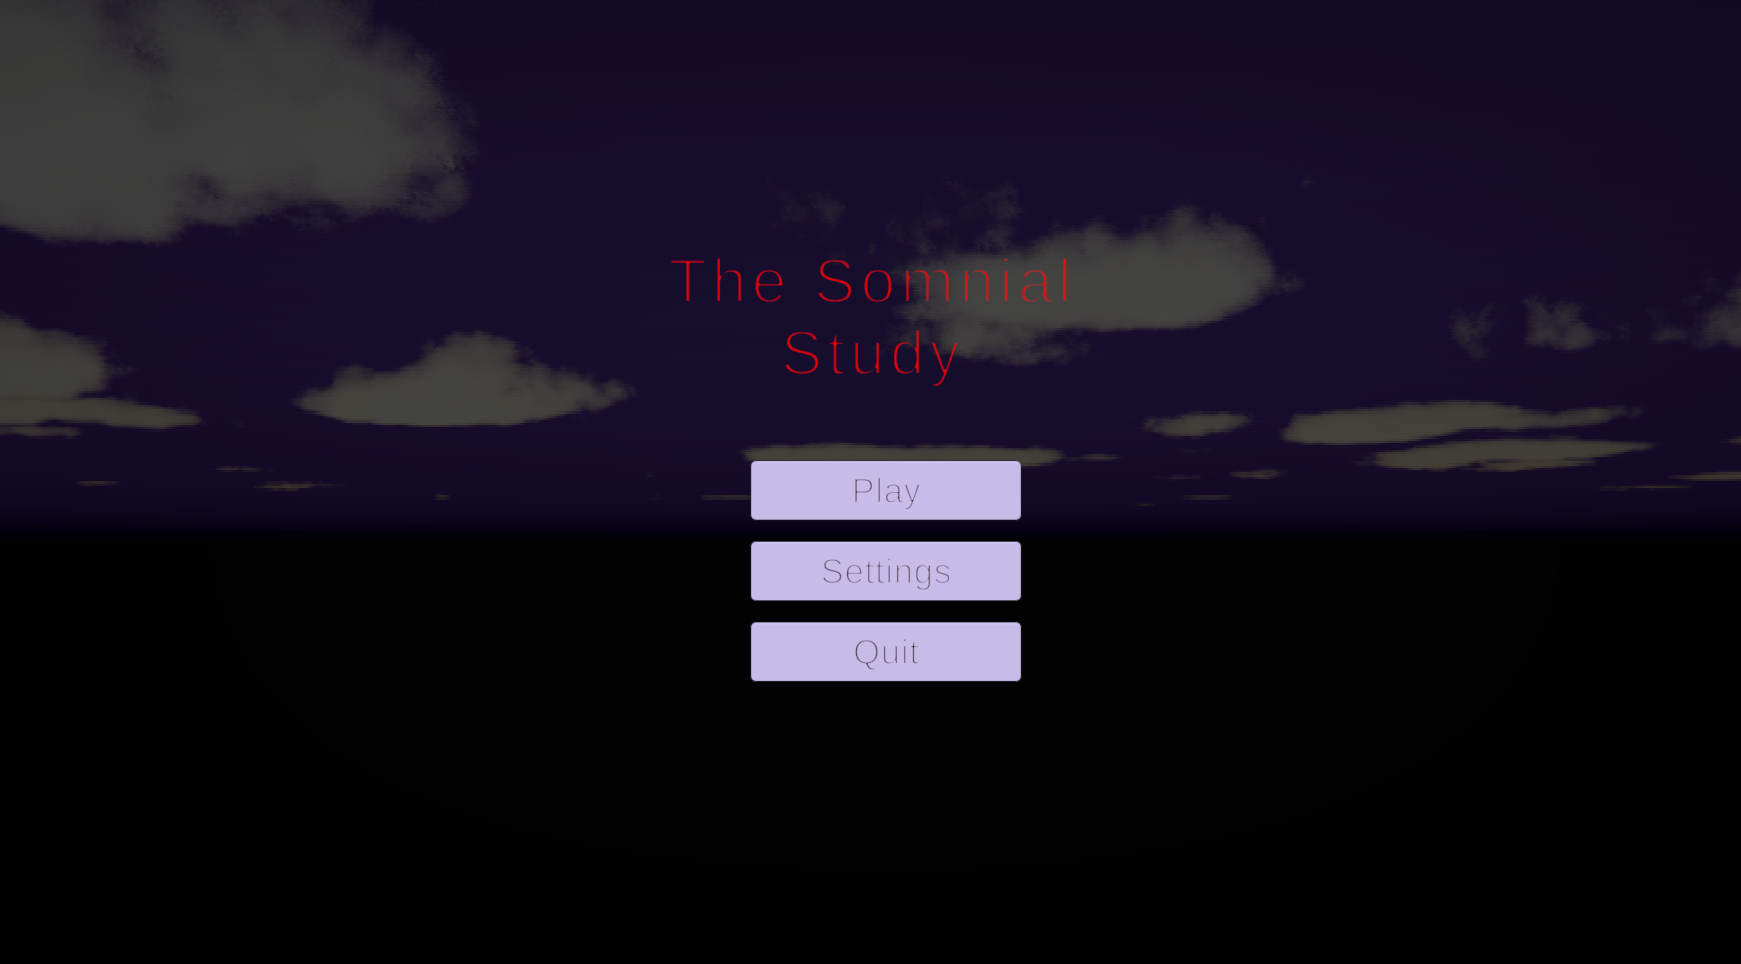
\includegraphics[width=\textwidth]{Menu.png}}
\vspace{0.2cm}
\textbf{Main Menu}
\end{minipage}
\hfill
\begin{minipage}{0.48\textwidth}
\centering
\fbox{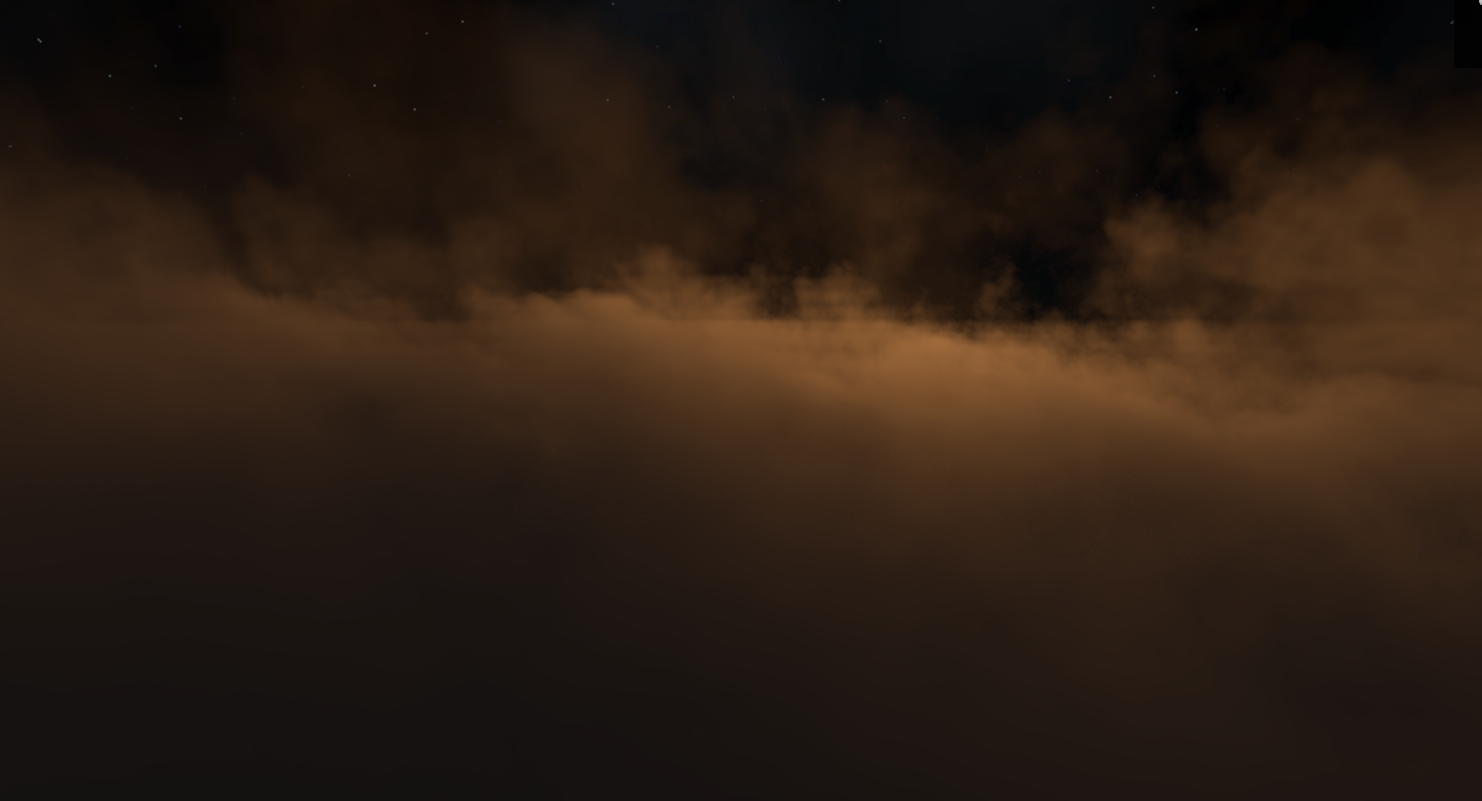
\includegraphics[width=\textwidth]{Clouds.png}}
\vspace{0.2cm}
\textbf{Volumetric Clouds}
\end{minipage}
\end{center}

\vspace{0.5cm}

% Row 2: Piano and Chase
\begin{center}
\begin{minipage}{0.48\textwidth}
\centering
\fbox{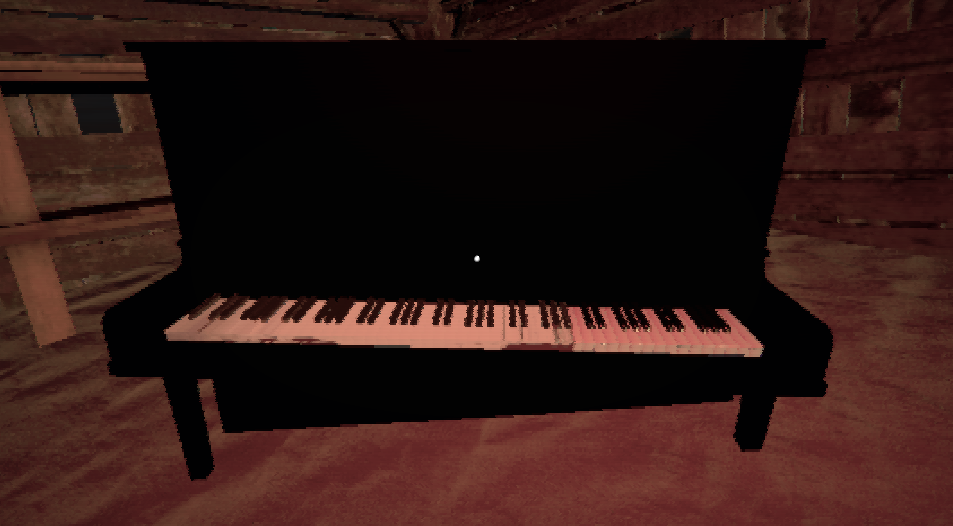
\includegraphics[width=\textwidth]{Piano.png}}
\vspace{0.2cm}
\textbf{Piano Dream}
\end{minipage}
\hfill
\begin{minipage}{0.48\textwidth}
\centering
\fbox{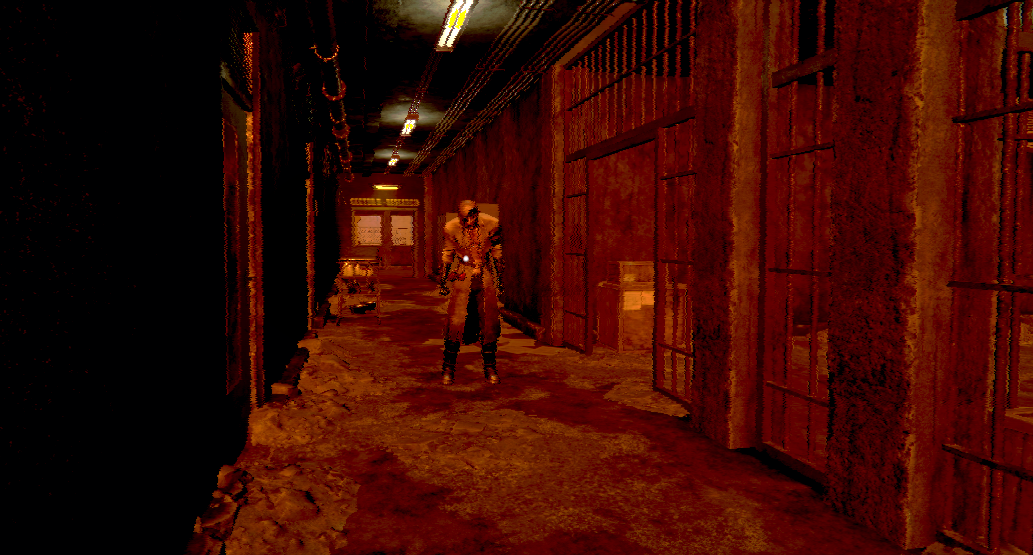
\includegraphics[width=\textwidth]{Chase.png}}
\vspace{0.2cm}
\textbf{Chase Sequence}
\end{minipage}
\end{center}

\vspace{0.5cm}

% Row 3: Opening (larger, featured)
\begin{center}
\fbox{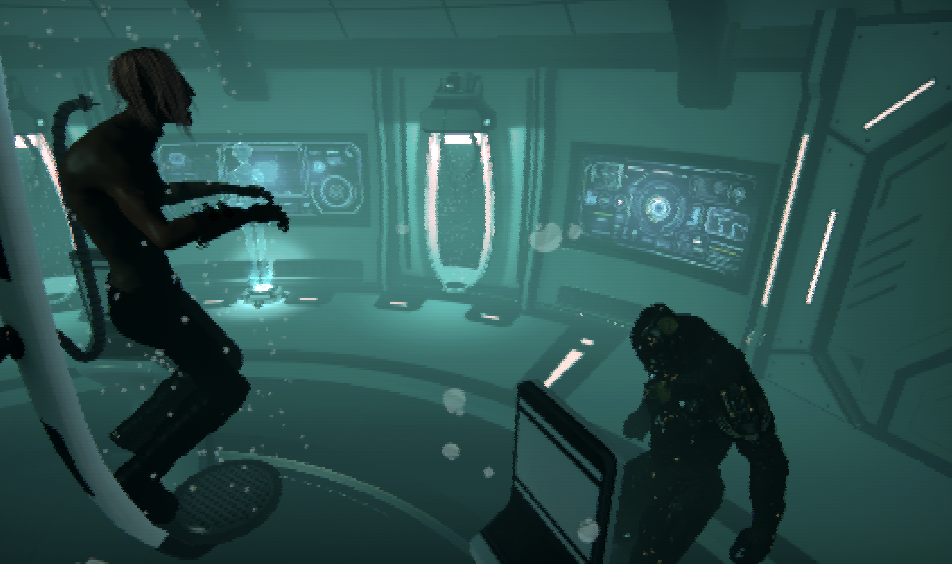
\includegraphics[width=0.95\textwidth]{Opening.png}}
\vspace{0.2cm}
\textbf{\large Opening Scene} --- The alien research facility
\end{center}

\end{posterblock}

\end{column}

\separatorcolumn

% =========================================
% COLUMN 3 - Features & Conclusion
% =========================================
\begin{column}{\colwidth}

\begin{posterblock}[Key Features]
\large

\textbf{First-Person Exploration \& Combat}\\
Environmental storytelling through logs and interactive objects, with planned boss encounters and combat mechanics for future updates.

\vspace{0.6cm}

\textbf{Volumetric Clouds \& Atmosphere}\\
Real-time volumetric cloud system with dynamic lighting, fog, and atmospheric scattering---one of my favorite visual elements to implement.

\vspace{0.6cm}

\textbf{Original Music \& Sound Design}\\
All music composed by me in Ableton Live, with state-driven audio layers that shift based on gameplay events.

\vspace{0.6cm}

\textbf{Custom Shaders \& Post-Processing}\\
CRT effects, glitch shaders, and dream distortion built in Unity's URP to create that unsettling, surreal atmosphere.

\vspace{0.6cm}

\textbf{AI State Machine}\\
Enemy AI with vision and hearing perception, NavMesh pathfinding, and multiple behavioral states for chase sequences.

\vspace{0.6cm}

\textbf{Interactive Puzzles}\\
Piano key sequences, object interactions, and audio cues that guide players through dream environments.

\end{posterblock}

\vspace{1cm}

\begin{posterblock}[Challenges \& Lessons Learned]
\large
\justifying
\textbf{Scene Management} was my biggest challenge. With scenes containing 17,000+ GameObjects, I had to build a custom scene optimizer with time-sliced loading to prevent frame hitches during transitions.

\vspace{0.5cm}
\textbf{Performance optimization} required implementing distance-based culling, throttled AI path updates, and careful management of when heavy operations run.

\vspace{0.5cm}
\textbf{Player controls} went through multiple iterations to get the physics-based movement feeling responsive without sliding.

\vspace{0.5cm}
This project taught me the importance of \textit{scope management} and building vertical slices early. What started as an ambitious idea had to be carefully scoped to be achievable as a solo developer.
\end{posterblock}

\vspace{0.8cm}

\begin{posterblock}[Future Plans]
\large
\textbf{December 2025:} Steam demo with the first dream sequence.\\[0.3cm]
\textbf{2026:} Full release with boss fights, expanded dreams, and polished gameplay.
\end{posterblock}

\end{column}

\separatorcolumn
\end{columns}

% ====================
% FOOTER
% ====================
\begin{tikzpicture}[remember picture,overlay]
  % Footer background
  \fill[chicowhite] (current page.south west) rectangle ([yshift=7cm]current page.south east);
  \draw[chicomaroon,line width=2pt] ([yshift=7cm]current page.south west) -- ([yshift=7cm]current page.south east);

  % Student info (bottom left)
  \node[anchor=south west,font=\Large,textdark] at ([xshift=3cm,yshift=1.5cm]current page.south west) {
    \begin{tabular}{@{}l@{}}
      \textbf{Developer:} Mustafa Ali \\[0.3cm]
      \textbf{Major:} Computer Science \\[0.3cm]
      \textbf{Department:} Computer Science
    \end{tabular}
  };

  % College of Engineering Logo (center)
  \node[anchor=south] at ([yshift=1cm]current page.south) {
    
\includegraphics[height=5cm]{Csu Chico College of Engineering Logo.jpg}
  };

  % Steam info (bottom right)
  \node[anchor=south east,font=\Large,textdark,align=right] at ([xshift=-3cm,yshift=1.5cm]current page.south east) {
    \begin{tabular}{@{}r@{}}
      \textbf{Platform:} Steam (PC) \\[0.3cm]
      \textbf{Demo Release:} December 2025 \\[0.3cm]
      \textbf{Engine:} Unity 6 (URP)
    \end{tabular}
  };

\end{tikzpicture}

\end{frame}
\end{document}
